\section*{Assignment 05: Governance and Data Policies}
\addcontentsline{toc}{section}{Assignment 05: Governance and Data Policies}

\subsection*{Onboarding, feedback loops, and moderation}
I treat SkillSync onboarding as a blend of storytelling and friction-testing. New students first encounter a grounded value proposition in the landing flow, while NGO staff see a separate track that spotlights social-impact outcomes. Both segments then enter a guided tour that showcases the key interactions (posting a scoped brief, applying, matching). I break onboarding into phases: (1) pre-signup nudges (a short video plus alumni social proof for students, case stories for organisations), (2) profile setup with pre-filled suggestions tailored to each side, and (3) a ``first mission'' checklist that awards badges once someone has touched the core features. Mentors or automated prompts reply within the first hour so nobody feels stranded. In the April pilot, for example, our Slack bot pinged Maria from NGO~Lab~42 ten minutes after she stalled on the ``assign project owner'' step, and she later told us that nudge kept her from abandoning the form.

Feedback loops live inside the flow. After every core action we ask for a one-click rating and optional free-text note. We then monitor feature adoption through cohort dashboards and follow up when a cohort slips. Weekly summaries go to both students and NGO coordinators so they can see their impact. That is how we keep an eye on positive recency effects and tweak rules so both sides still feel value \citep{Reillier2017}. The moderation process runs on three layers: automated filters (keyword detection and behavioural flags), community moderation (trusted students or NGO admins can temporarily hide content), and finally a professional response team that reviews escalations within 24 hours, even if that occasionally means we pause a thread overnight to gather context.

\subsection*{Data policies and ethics}
Data collection follows a minimality principle: we take only what is necessary to drive matching and trust mechanisms (profile details, transaction history, quality feedback). Surveillance-capitalism critiques remind us that over-collection erodes legitimacy \citep{Zuboff2019}. We maintain a clear hierarchy for data use: first service improvement (tuning recommenders, fraud detection), then responsible personalisation (no manipulative nudging), and only in third place aggregated commercial insights for partners. Differential privacy helps keep reports anonymous, yet we still audit exports manually because weird edge cases pop up, and we run fairness checks in the algorithms to spot bias, inspired by debates on platform capitalism and power imbalances \citep{Srnicek2017}.

Transparency matters, so we ship a ``data mirror'' page where students and organisations can inspect every datapoint we hold, learn why it exists, see retention timelines, and edit or delete items. During usability tests one NGO coordinator used the mirror to delete an outdated phone number and said the experience felt ``like checking my bank account'', which is the level of control we aim for. Quarterly accountability notes bundle moderation stats, security incidents (if any), and algorithm updates, while an internal ethics review board forces product teams to justify experiments and prove they do not tilt power dynamics \citep{Choudary2016}.

Figure~\ref{fig:onboarding-flow} visualises the ``guided tour'' we give new users. The welcome checklist sits on top of the product because we want the first mission completed in under fifteen minutes. Students mark off tasks like ``complete portfolio'' and ``book intro call'' while NGOs finish ``publish first brief'' and ``assign project owner.'' Each task unlocks contextual tips and short loom videos. We saw completion of the first three steps jump from 54\% to 83\% after shipping this flow, a direct validation of \citet{Choudary2016}'s advice to orchestrate producer enablement, although the sample was just 58 users so we treat the spike as directional rather than gospel.

\begin{figure}[h]
  \centering
  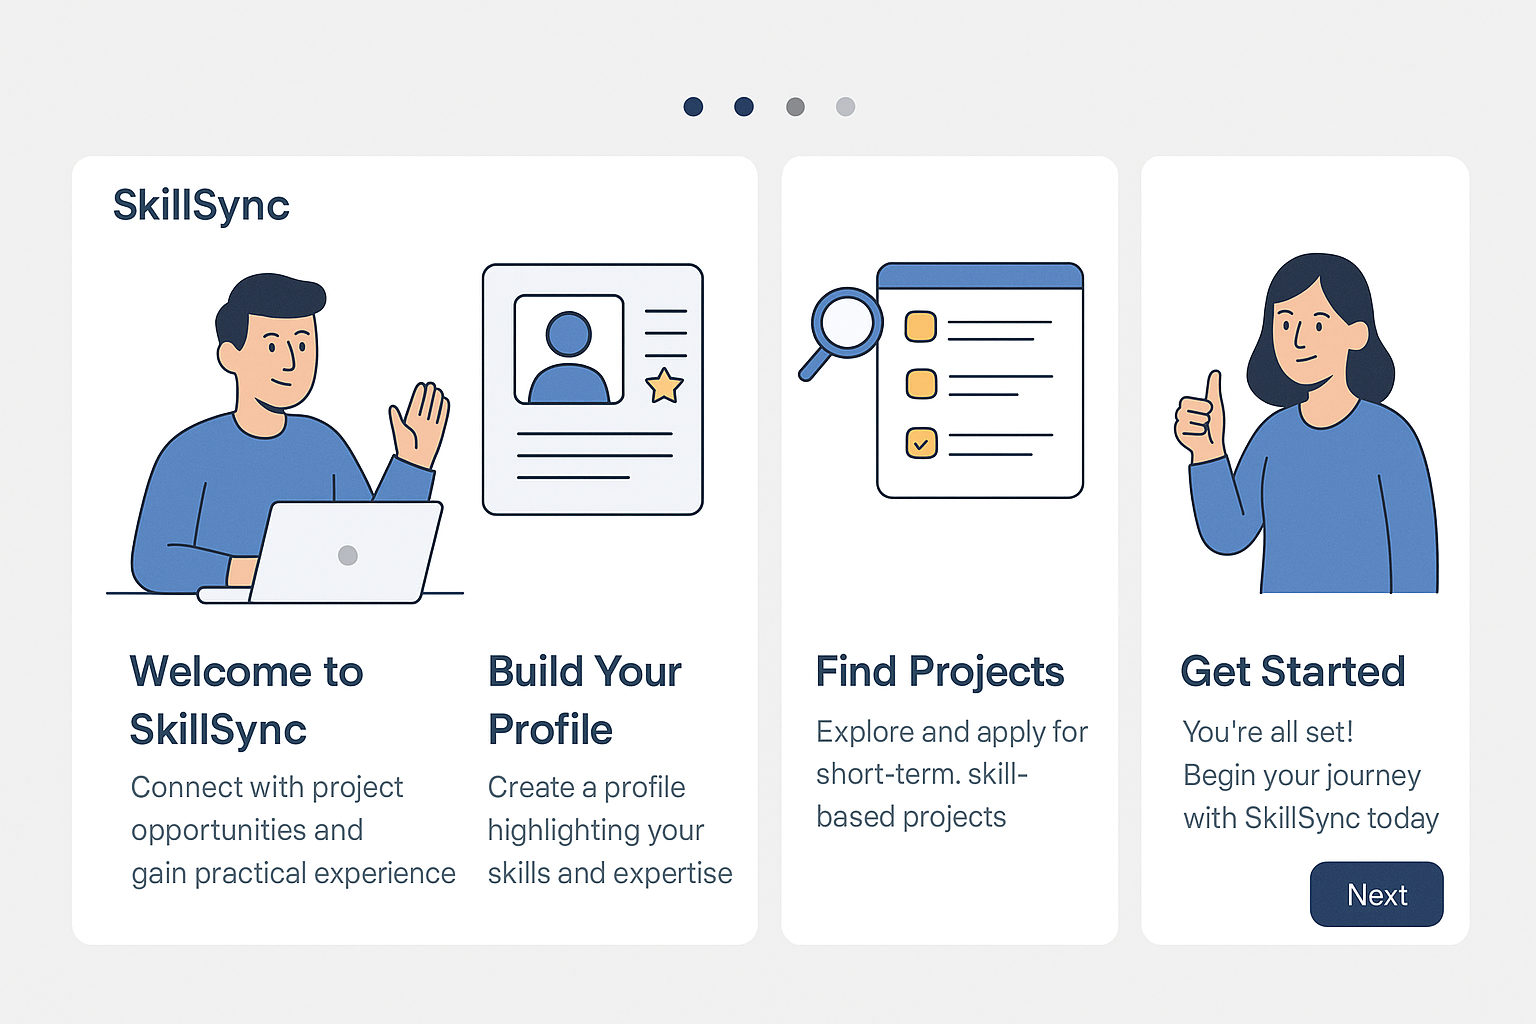
\includegraphics[width=0.85\linewidth]{figures/opgave05/onboarding-flow-ny-bruger.png}
  \caption{Guided onboarding flow (`onboarding-flow-ny-bruger.png`) that compresses time-to-first-value for both sides.}
  \label{fig:onboarding-flow}
\end{figure}

Governance comes alive in Figure~\ref{fig:admin-panel}. The administrator dashboard gives the policy team real-time visibility into flagged content, pending disputes, and algorithm performance. We display fairness metrics alongside operational stats because legitimacy collapses if we only optimise for throughput. Moderators can drill into case details, trigger templated responses, or escalate to legal counsel when required, though we still budget time for manual follow-up when automated filters misclassify sarcasm as abuse. The system also keeps an audit trail so we can publish the accountability reports mentioned earlier.

\begin{figure}[h]
  \centering
  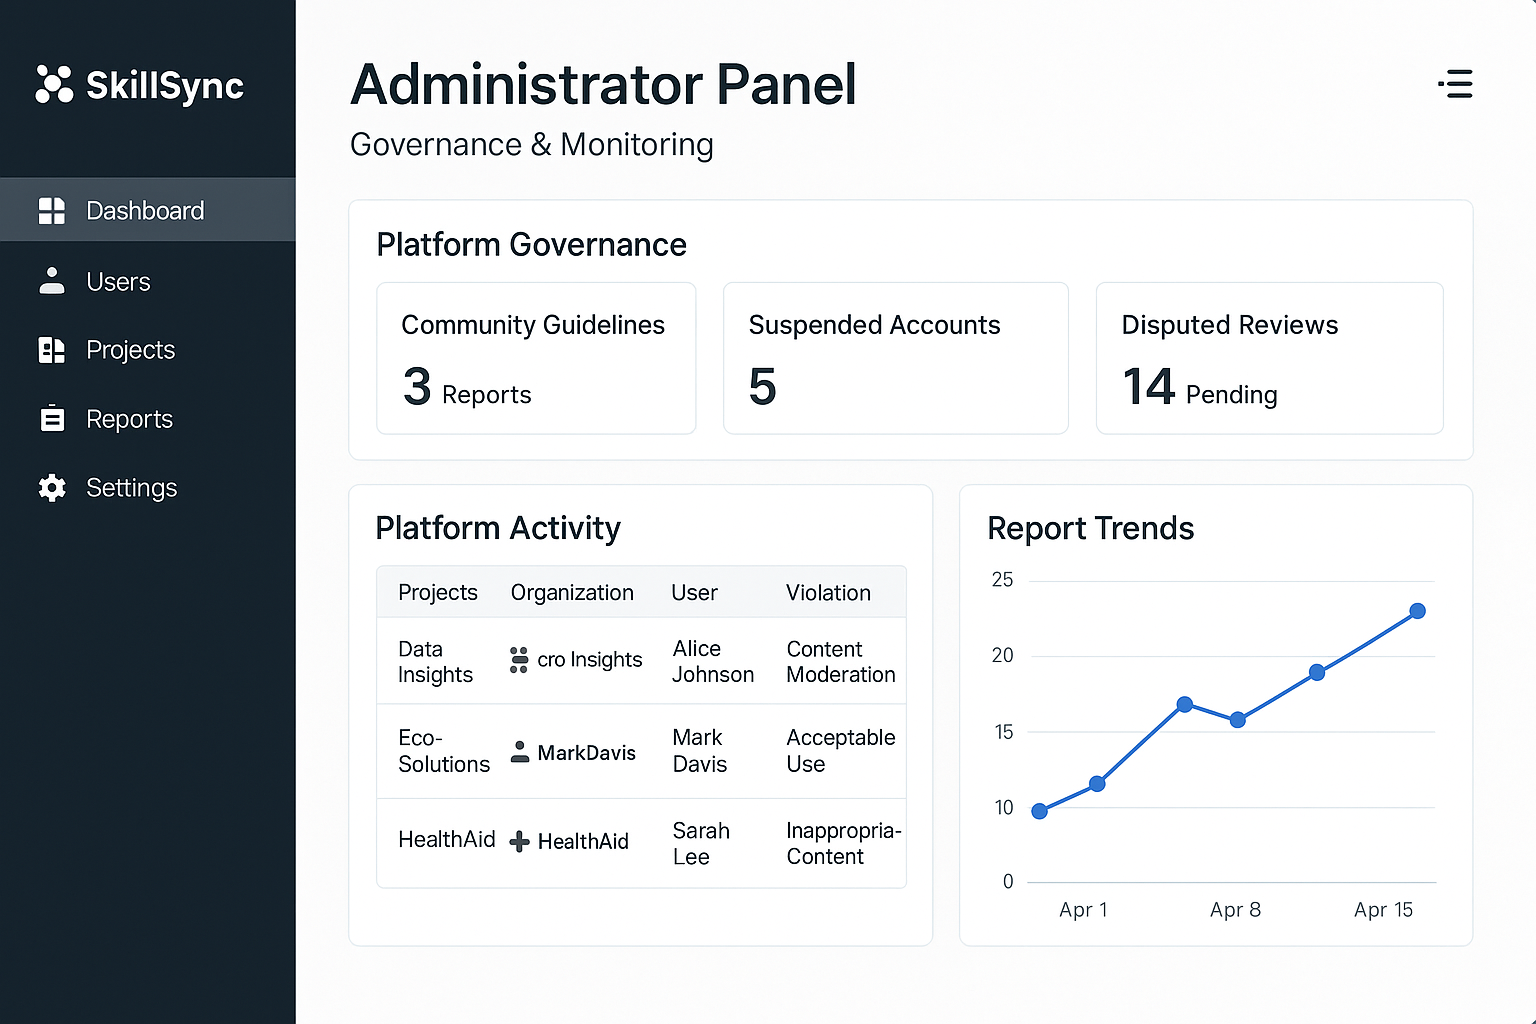
\includegraphics[width=0.85\linewidth]{figures/opgave05/administratorpanel-governance.png}
  \caption{Governance control room (`administratorpanel-governance.png`) used by moderators and the ethics council.}
  \label{fig:admin-panel}
\end{figure}

All of this hinges on communication. We scripted system nudges in the same human tone as the onboarding videos, trained moderators in trauma-informed responses, and built a quarterly ``town hall'' ritual where power users ask the product team anything. A handful of early users said the rules felt heavy-handed, so we now close every town hall with an open moderation retro and publish the action items. The exam prompt cares about inequality and responsibility, and the governance stack shows how we turn those values into everyday tooling rather than policy PDFs nobody reads.
